\documentclass[12pt]{article}
\usepackage{hyperref}
\usepackage{listings}
\usepackage[margin=1in]{geometry}
\usepackage{enumitem}
\usepackage{multicol}
\usepackage{array}
\usepackage{titlesec}
\usepackage{helvet}
\renewcommand{\familydefault}{\sfdefault}
\usepackage{amsmath}     % For math equations
\usepackage{amssymb}     % For advanced math symbols
\usepackage{amsfonts} % For math fonts
\usepackage{gvv}
\usepackage{esint}
\usepackage[utf8]{inputenc}
\usepackage{graphicx}
\usepackage{pgfplots}
\pgfplotsset{compat=1.18}
\titleformat{\section}{\bfseries\large}{\thesection.}{1em}{}
\setlength{\parindent}{0pt}
\setlength{\parskip}{6pt}
\usepackage{multirow}
\usepackage{float}
\usepackage{caption}


\begin{document}

\textbf{Problem 5.13.18.} 

If the system of linear equations
\begin{align}
x + ky + 3z &= 0, \\
3x + ky - 2z &= 0, \\
2x + 4y - 3z &= 0
\end{align}
has a non-zero solution $(x,y,z)$, then $\dfrac{xz}{y^2}$ is equal to
\begin{align}
\text{a) } 10 \quad \text{b) } -30 \quad \text{c) } 30 \quad \text{d) } -10
\end{align}

\bigskip
\textbf{Input Variables:}

\begin{table}[H]
\centering
\begin{tabular}{|c|c|}
\hline
\textbf{Variable} & \textbf{Description} \\
\hline
$x,y,z$ & Unknowns of the system \\
\hline
$k$ & Parameter in the system \\
\hline
\end{tabular}
\end{table}

\bigskip
\textbf{Solution:}

Start with the augmented matrix:
\begin{align}
\myvec{1 & k & 3 & 0 \\ 3 & k & -2 & 0 \\ 2 & 4 & -3 & 0}.
\end{align}

Eliminating below the first pivot:
\begin{align}
R_2 \to R_2 - 3R_1,\quad R_3 \to R_3 - 2R_1
\;\Rightarrow\;
\myvec{1 & k & 3 & 0 \\ 0 & -2k & -11 & 0 \\ 0 & 4-2k & -9 & 0}.
\end{align}

Next, remove the second entry in row 3:
\begin{align}
R_3 \to R_3 + \Big(\tfrac{2}{k}-1\Big)R_2
\;\Rightarrow\;
\myvec{1 & k & 3 & 0 \\ 0 & -2k & -11 & 0 \\ 0 & 0 & \tfrac{2(k-11)}{k} & 0}.
\end{align}

For a homogeneous system $A\vec{v}=0$, a non-trivial solution exists only if $\operatorname{rank}(A)<3$.  
Hence the last pivot must vanish:
\begin{align}
\dfrac{2(k-11)}{k}=0 \;\Rightarrow\; k=11.
\end{align}

Substitute $k=11$:
\begin{align}
\myvec{1 & 11 & 3 & 0 \\ 3 & 11 & -2 & 0 \\ 2 & 4 & -3 & 0}
\;\longrightarrow\;
\myvec{1 & 11 & 3 & 0 \\ 0 & 2 & 1 & 0 \\ 0 & 0 & 0 & 0}.
\end{align}

From row 2: $2y+z=0 \Rightarrow z=-2y$.  \\
From row 1: $x+11y+3z=0 \Rightarrow x=-5y$.

\begin{align}
\vec{v} = y\myvec{-5\\1\\-2}, \quad y\neq 0.
\end{align}

Finally,
\begin{align}
\frac{xz}{y^2} = \frac{(-5y)(-2y)}{y^2} = 10.
\end{align}

\begin{align}
\boxed{10}
\end{align}

\begin{figure}[H]
    \centering
    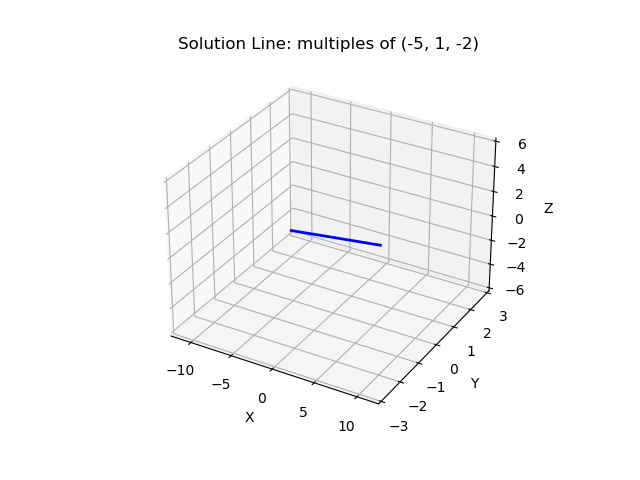
\includegraphics[width=0.9\columnwidth]{figs/solvek.png}
    \caption{}
    \label{fig:placeholder}
\end{figure}


\end{document}
